%   ------------------------------------------------------------------------
\FloatBarrier
\section{ChatGPT}
\label{s.chatGPTApendice}


\begin{figure}[htbp]
    \centering
    \caption{\small Processo da utilização 1 do chatGPT em julho/2025}
    \label{fig:chatGPT1}

    \begin{subfigure}{0.75\linewidth}
        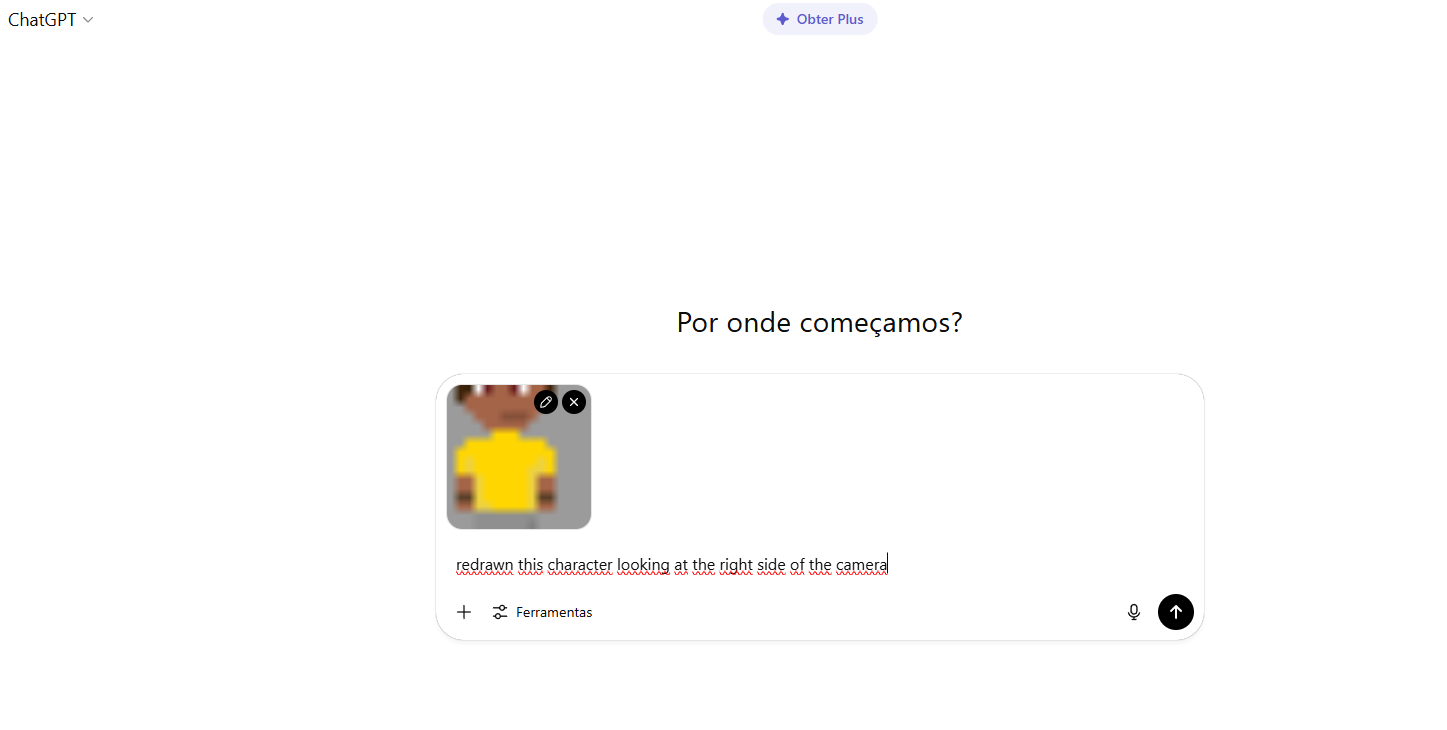
\includegraphics[width=1\linewidth]{figs/chatGPT/visao_lateral/tela1_pixel.PNG}
        \caption{\small Prompt e arquivos anexados}
        \label{fig:chatGPT1a}
    \end{subfigure}
    \begin{subfigure}{0.2\linewidth}
        
\includegraphics[width=1\linewidth]{figs/chatGPT/visao_lateral/res1_pixel.png}
        \caption{\small Sprite gerado}
        \label{fig:chatGPT1b}
    \end{subfigure}
        \begin{subfigure}{0.75\linewidth}
        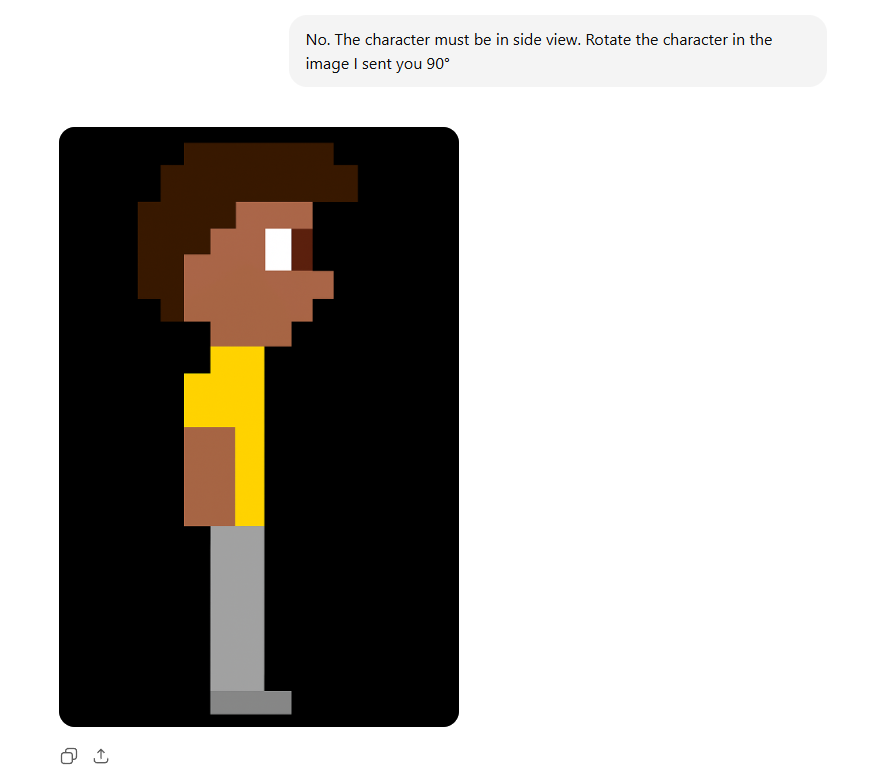
\includegraphics[width=1\linewidth]{figs/chatGPT/visao_lateral/tela2_pixel.PNG}
        \caption{\small Reformulação do prompt}
        \label{fig:chatGPT1c}
    \end{subfigure}
    \legend{\small Fonte: Elaborada pela autora, utilizando a ferramenta chatGPT.}
\end{figure}

\begin{figure}[htbp]
    \centering
    \caption{\small Processo da utilização 2 do chatGPT em julho/2025}
    \label{fig:chatGPT2}

    \begin{subfigure}{0.75\linewidth}
        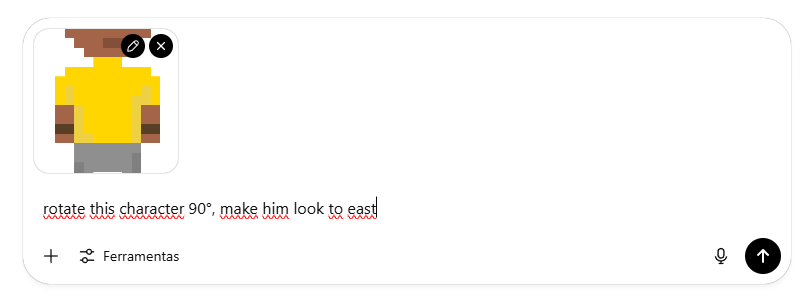
\includegraphics[width=1\linewidth]{figs/chatGPT/visao_lateral/tela1.PNG}
        \caption{\small Prompt e arquivos anexados}
        \label{fig:chatGPT2a}
    \end{subfigure}
    \begin{subfigure}{0.2\linewidth}
        
\includegraphics[width=1\linewidth]{figs/chatGPT/visao_lateral/res1.png}
        \caption{\small Sprite gerado}
        \label{fig:chatGPT2b}
    \end{subfigure}
        \begin{subfigure}{0.65\linewidth}
        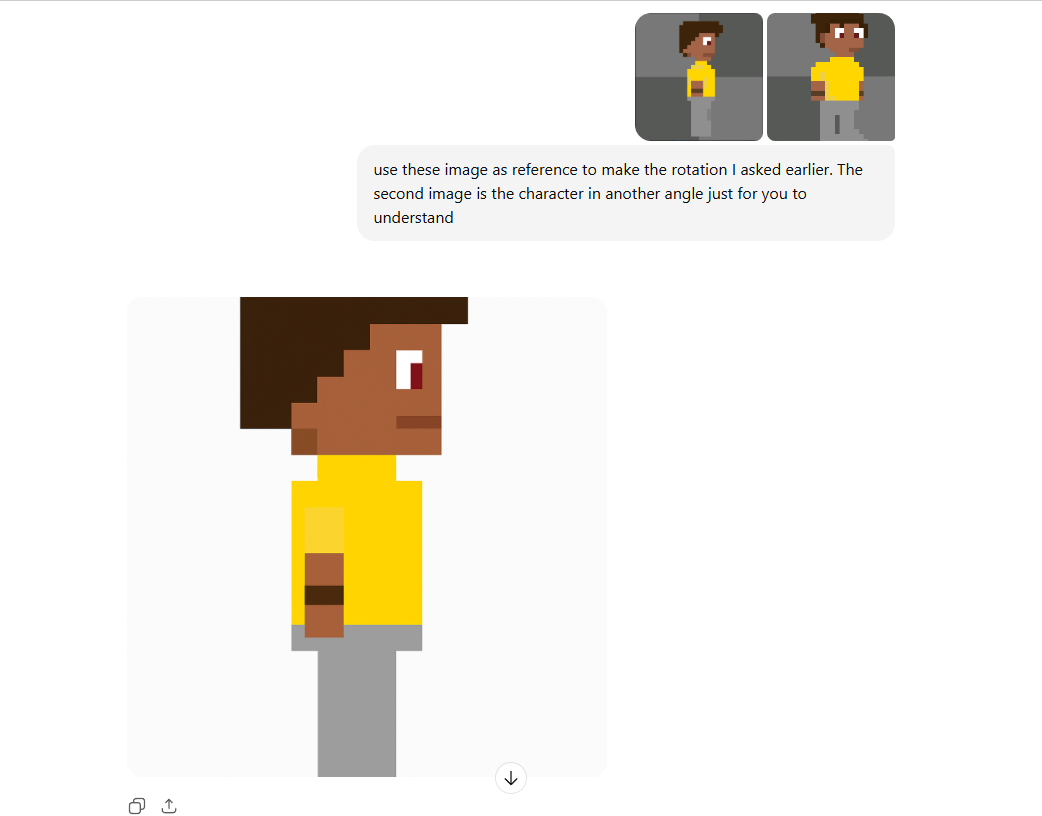
\includegraphics[width=1\linewidth]{figs/chatGPT/visao_lateral/tela2.PNG}
        \caption{\small Novos arquivos anexados para contexto}
        \label{fig:chatGPT2c}
    \end{subfigure}
    \begin{subfigure}{0.55\linewidth}
        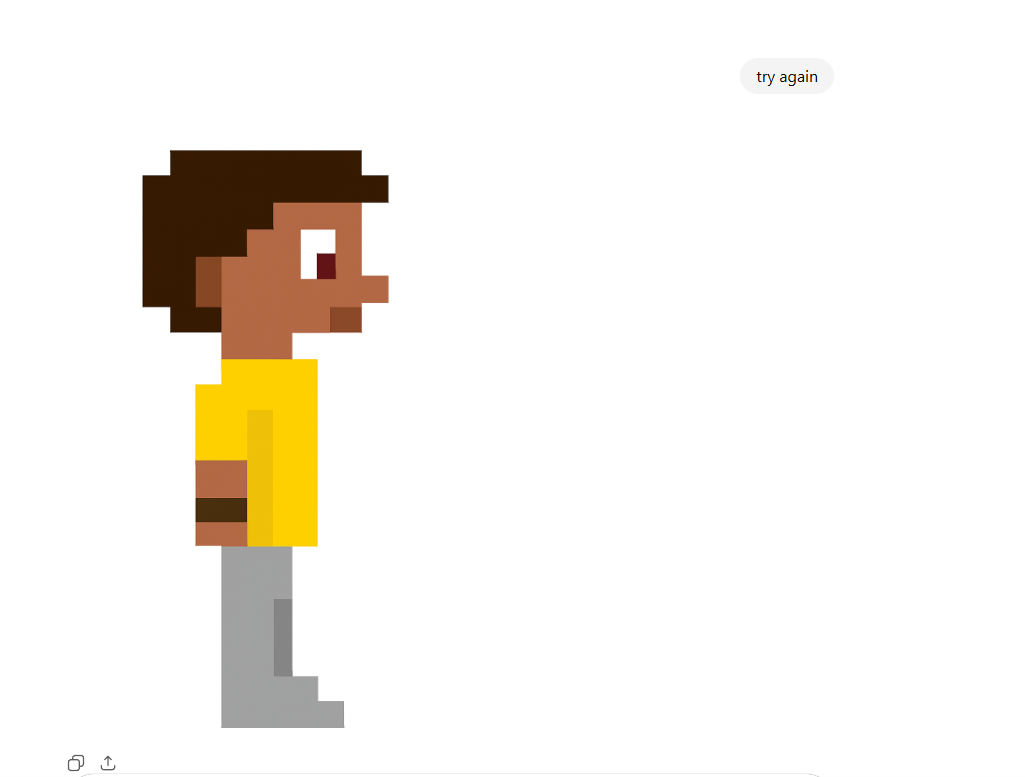
\includegraphics[width=1\linewidth]{figs/chatGPT/visao_lateral/tela 2.5.PNG}
        \caption{\small Re geração}
        \label{fig:chatGPT2d}
    \end{subfigure}
    \legend{\small Fonte: Elaborada pela autora, utilizando a ferramenta chatGPT.}
\end{figure}

\begin{figure}[htbp]
    \centering
    \caption{\small Processo da utilização 3 do chatGPT em julho/2025}
    \label{fig:chatGPT3}

    \begin{subfigure}{0.75\linewidth}
        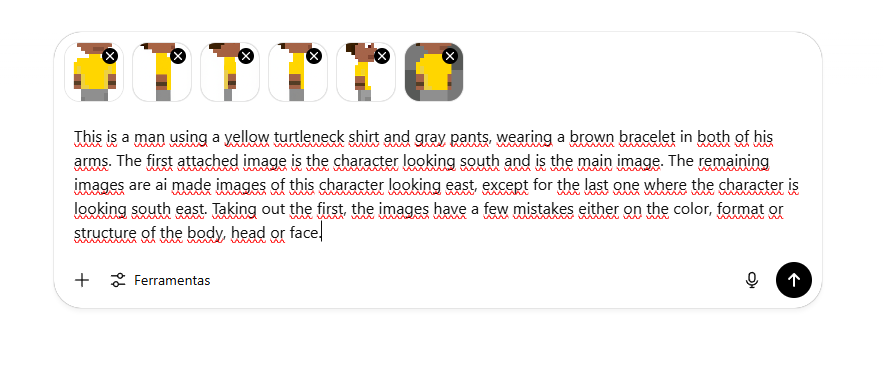
\includegraphics[width=1\linewidth]{figs/chatGPT/visao_lateral/tela3.PNG}
        \caption{\small Contextualização e arquivos anexados}
        \label{fig:chatGPT3a}
    \end{subfigure}
    \begin{subfigure}{0.75\linewidth}
        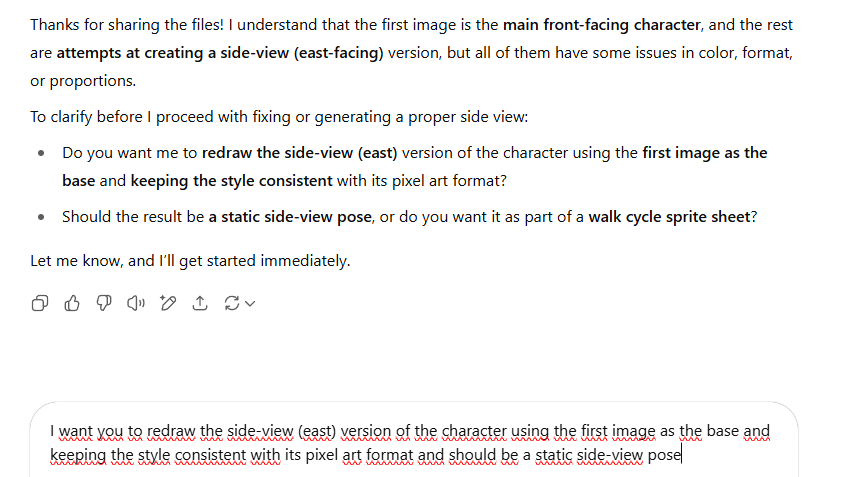
\includegraphics[width=1\linewidth]{figs/chatGPT/visao_lateral/tela4.PNG}
        \caption{\small Prompt}
        \label{fig:chatGPT3b}
    \end{subfigure}
        \begin{subfigure}{0.2\linewidth}
        
\includegraphics[width=1\linewidth]{figs/chatGPT/visao_lateral/res4.PNG}
        \caption{\small Imagem gerada}
        \label{fig:chatGPT3c}
    \end{subfigure}
    \begin{subfigure}{0.55\linewidth}
        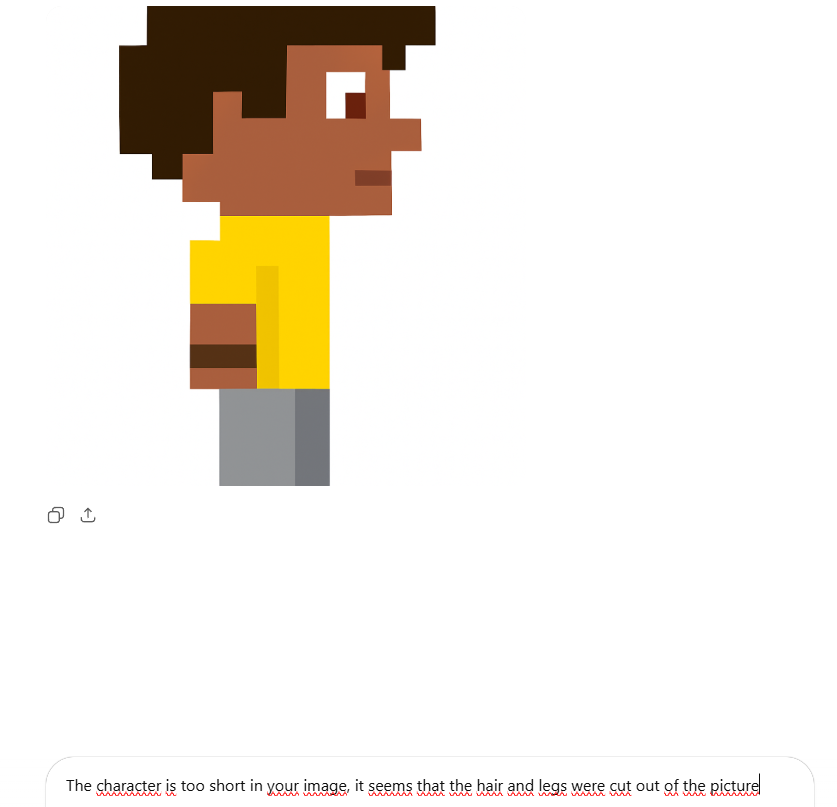
\includegraphics[width=1\linewidth]{figs/chatGPT/visao_lateral/tela5.PNG}
        \caption{\small Prompt para correção de erro}
        \label{fig:chatGPT3d}
    \end{subfigure}
    \begin{subfigure}{0.2\linewidth}
        
\includegraphics[width=1\linewidth]{figs/chatGPT/visao_lateral/res5.PNG}
        \caption{\small Imagem gerada}
        \label{fig:chatGPT3e}
    \end{subfigure}
    \legend{\small Fonte: Elaborada pela autora, utilizando a ferramenta chatGPT.}
\end{figure}

\begin{figure}[htbp]
    \centering
    \caption{\small Processo da utilização do chatGPT em junho/2025}
    \label{fig:chatGPT4}

    \begin{subfigure}{0.75\linewidth}
        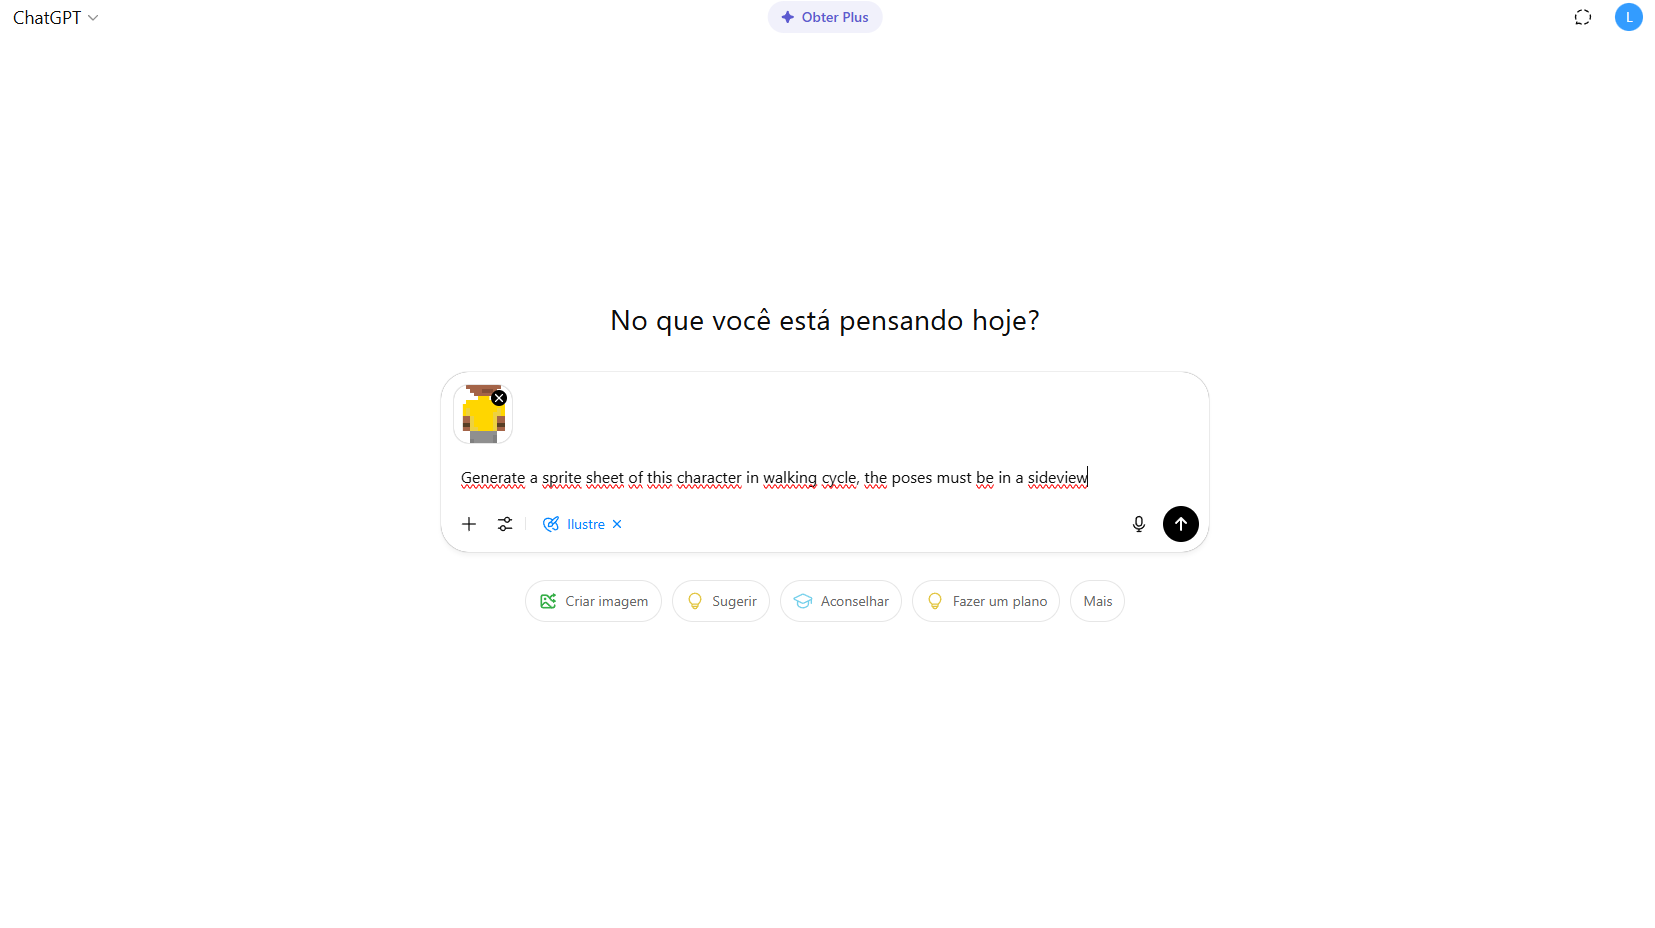
\includegraphics[width=1\linewidth]{figs/chatGPT/walking_cycle/front_view/tela.PNG}
        \caption{\small Prompt e arquivo anexado}
        \label{fig:chatGPT4a}
    \end{subfigure}
    \begin{subfigure}{0.2\linewidth}
        
\includegraphics[width=1\linewidth]{figs/chatGPT/walking_cycle/front_view/walking cycle 1.png}
        \caption{\small Imagem gerada}
        \label{fig:chatGPT4b}
    \end{subfigure}
    \begin{subfigure}{0.65\linewidth}
        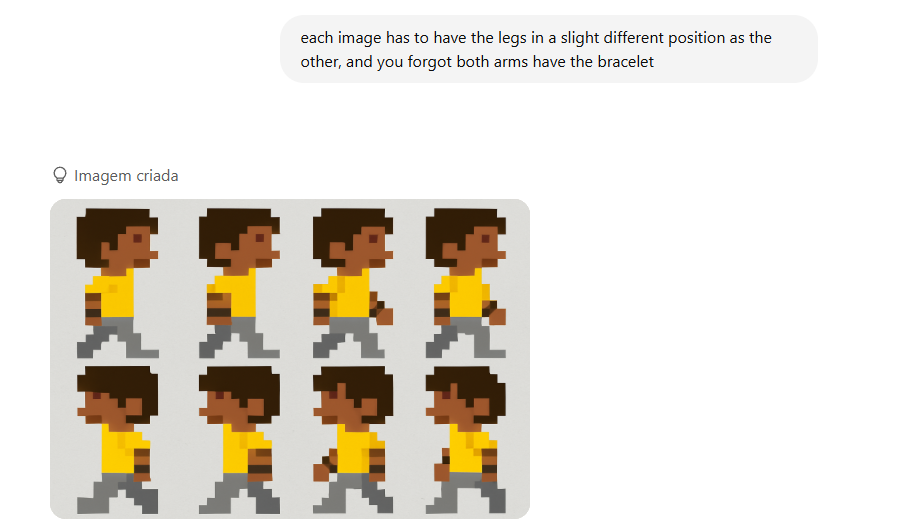
\includegraphics[width=1\linewidth]{figs/chatGPT/walking_cycle/front_view/tela2.PNG}
        \caption{\small Prompt para correção de erros}
        \label{fig:chatGPT4c}
    \end{subfigure}
        \begin{subfigure}{0.55\linewidth}
        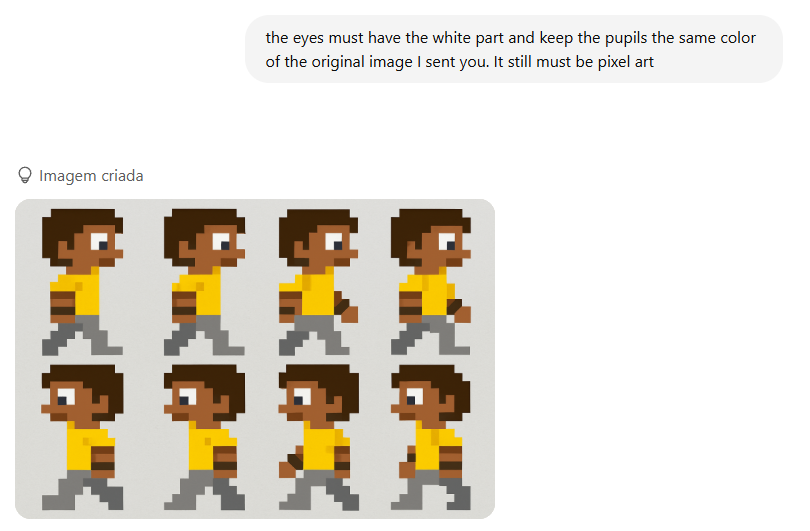
\includegraphics[width=1\linewidth]{figs/chatGPT/walking_cycle/front_view/tela3.PNG}
        \caption{\small Prompt final}
        \label{fig:chatGPT4d}
    \end{subfigure}

    \legend{\small Fonte: Elaborada pela autora, utilizando a ferramenta chatGPT.}
\end{figure}

\begin{figure}[htbp]
    \centering
    \caption{\small Processo da utilização 4 do chatGPT em julho/2025}
    \label{fig:chatGPT5}

    \begin{subfigure}{1\linewidth}
        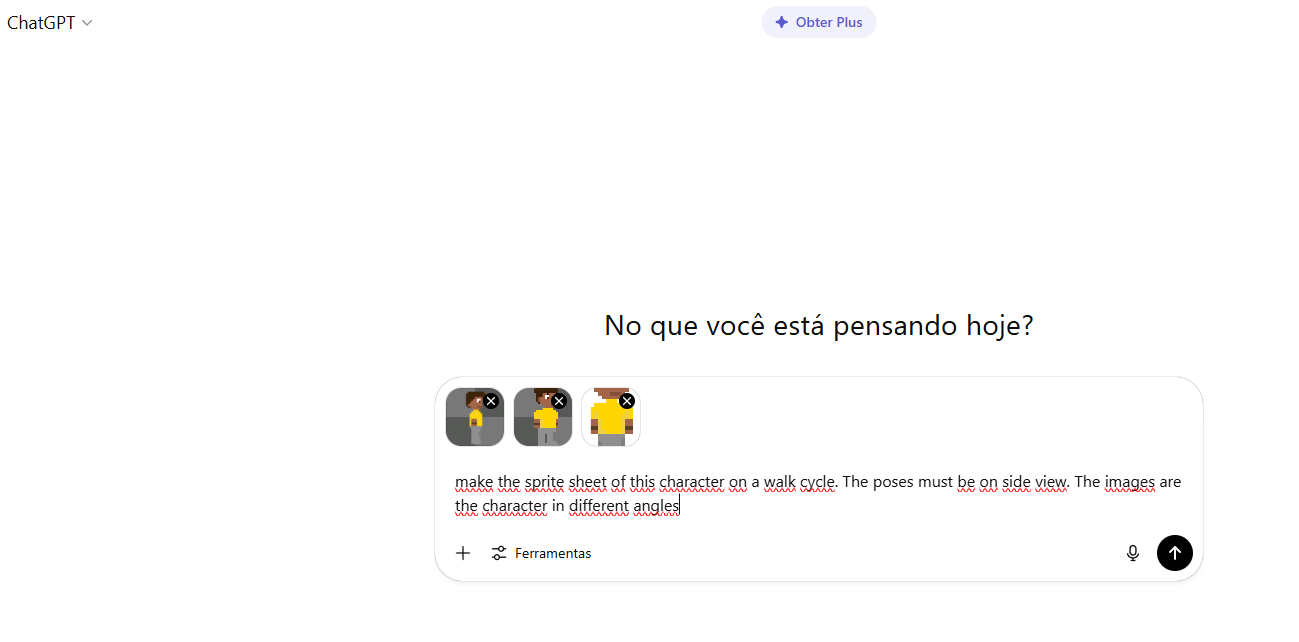
\includegraphics[width=1\linewidth]{figs/chatGPT/walking_cycle/side_view/tela1.PNG}
        \caption{\small Prompt e arquivos anexados}
        \label{fig:chatGPT5a}
    \end{subfigure}

    \begin{subfigure}{0.5\linewidth}
        
\includegraphics[width=1\linewidth]{figs/chatGPT/walking_cycle/side_view/walking cycle 1.png}
        \caption{\small Imagem gerada}
        \label{fig:chatGPT5b}
    \end{subfigure}
    \legend{\small Fonte: Elaborada pela autora, utilizando a ferramenta chatGPT.}
\end{figure}

\begin{figure}[htbp]
    \centering
    \caption{\small Processo da utilização 5 do chatGPT em julho/2025}
    \label{fig:chatGPT6}

    \begin{subfigure}{1\linewidth}
        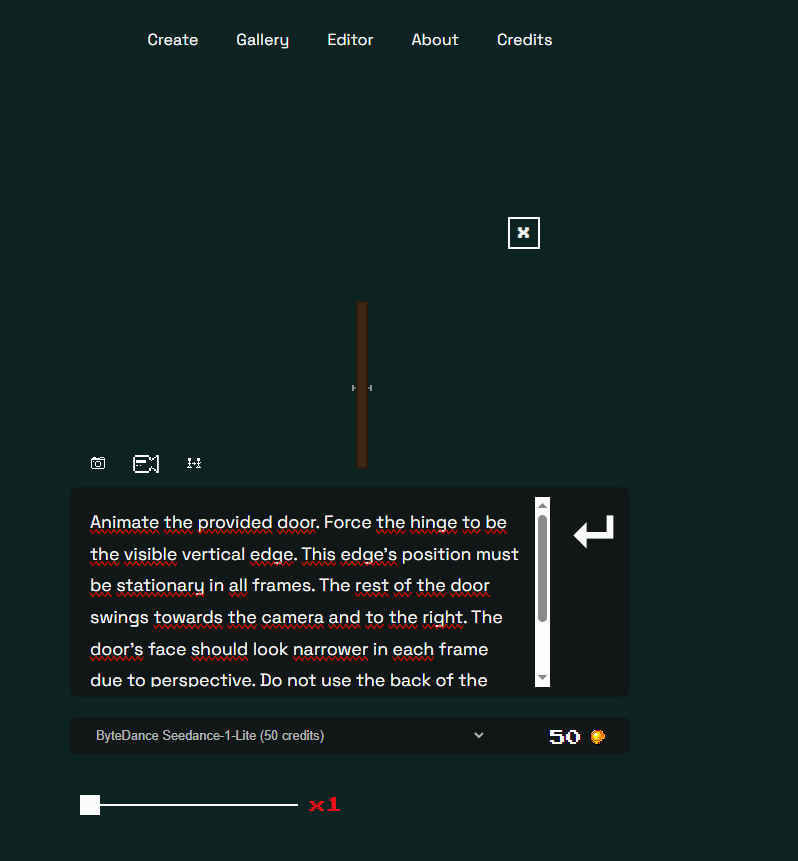
\includegraphics[width=1\linewidth]{figs/chatGPT/walking_cycle/side_view/tela3.PNG}
        \caption{\small Prompt e arquivos anexados}
        \label{fig:chatGPT6a}
    \end{subfigure}

    \begin{subfigure}{0.5\linewidth}
        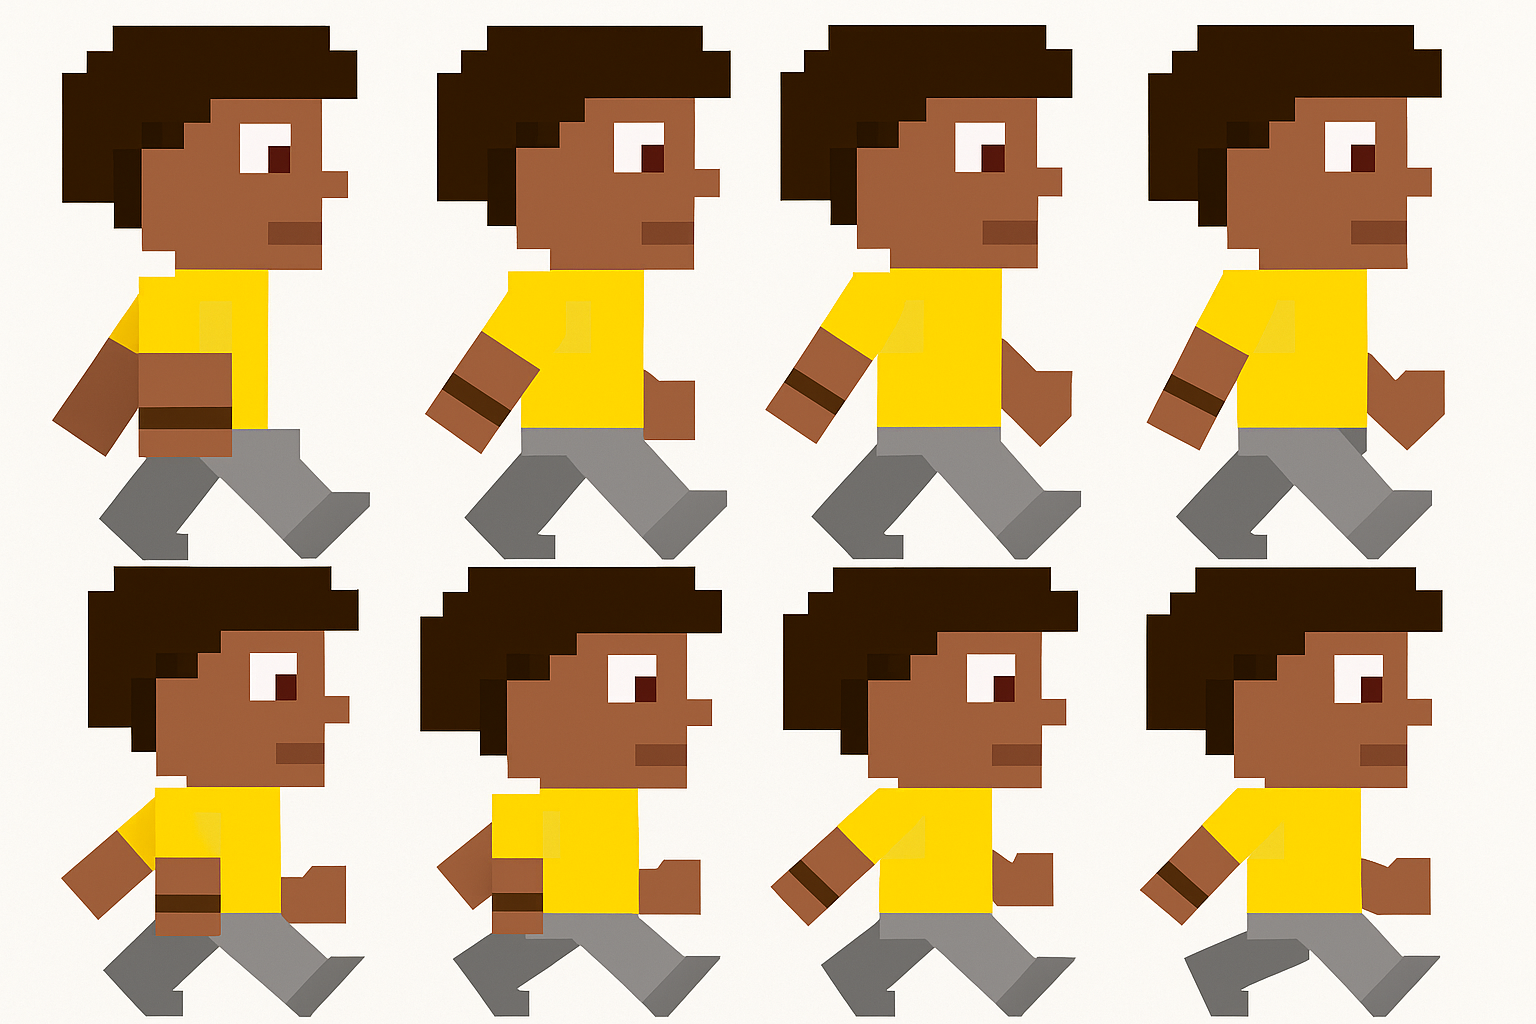
\includegraphics[width=1\linewidth]{figs/chatGPT/walking_cycle/side_view/walking cycle 2.png}
        \caption{\small Imagem gerada}
        \label{fig:chatGPT6b}
    \end{subfigure}
    \legend{\small Fonte: Elaborada pela autora, utilizando a ferramenta chatGPT.}
\end{figure}